\documentclass{article}
\usepackage{standalone}
\graphicspath{{Images/}}
\usepackage[e]{Template/gameshf}
\usepackage{import}

%opening
\title{STEM games 2019}
\author{Mentori}

\begin{document}
	
	\maketitle
	
	
	
	\section{Introduction}
	
	The choice of propulsion system type is one of the most important parts in submarine’s design process since it determines the ability of fulfilling its purpose. Submarines that perform underwater research activities require endurance and certain flexibility in different littoral conditions. For example, conventional motor propulsion systems, such as diesel electric, when operational, require fresh air intake for driving electrical generator. In this way, a period while a submarine can remain submerged is limited by the power and endurance of the battery system and counts in hours or few days at most. Therefore, when it comes to endurance such systems might not be an optimal choice. Technology that overcomes this drawback is a nuclear power system which offers better endurance (even few months) and speed of the submarines but there are number of disadvantages (very expensive, operational limitations in shallow littoral waters etc.) that make them unsuitable for underwater research activities. The most suitable seems to be so called Air Independent Propulsion systems (AIP systems) which are marine propulsion technologies that allows non-nuclear submarine to operate without access to atmospheric oxygen. 
	
	One of the most interesting is definitely French AIP technology so called MESMA (Module d'Energie Sous-Marine Autonome). This is the AIP system that uses closed-turbine cycle for powering electrical generator and the heat for steam generation is provided by liquid ethanol (ili bioethanol) combustion in pure oxygen (sometimes mixed with argon). Combustion of pure ethanol (ili bioethanol) makes this system ecologically much more acceptable than other systems that use conventional fuels. In this way, virtually silent MESMA exploits all advantages of AIP systems for maintenance of underwater habitats and performing underwater research or training activities.
	 
	Today's assignment is to design a MESMA power generation system for submarine propulsion for a given submarine hull which consists of outer and inner shell, showed on Figure 1. Inside inner shell there is a reserved space of fixed volume (zadati ovdje ili zajedno sa skicom!) consisting of three compartments; fuel tanks compartment (Compartment 1), engineering room compartment (Compartment 2) and cargo place compartment (Compartment 3). Individual volumes of each compartment can be arbitrarily chosen but the sum of all compartment volumes is fixed to a constant value. 
	
	The scheme of MESMA power generation system is given in the assignment description and its performance (range, speed, efficiency, price?) (dopuniti, ako treba, kada tablica bodovanja bude gotova) will be evaluated for different depths according to the scoring table (možda nije dobar naziv) given later in the text. It is important to emphasize that one of evaluation categories is the size of the cargo place compartment so the care must be taken not to oversize the propulsion system which must be placed in other two compartments.
	
	The assignment can be divided into two steps: 
	
	\begin{enumerate}
		\item Design and dimension main components of the propulsion system,
		\item Define operational characteristics of some components.
	\end{enumerate}

	After the first step you will be given a full model of propulsion system with the components you selected which will help you define operational characteristics of some components.
	Detailed description of the system components is given in the next section.
	
	Engineers, good luck!
	
	Zadatak,
	Your task is to design submarine power generation system which can generate sufficient energy to travel xx km and generate minimum required power during xx hours when submarine is being loaded and unloaded.
	or: to design power generation system which can generate sufficient energy to travel 100 km at depth 50 m 20 km at depth  100 m and 20 km at depth 10 m
	Formule za nosivost, masu, otpor, maksimalna duljina izmjenjivača, maksimalna snaga turbine i drugo ovisno o veličini podmornice
		
		
	\section{Power generation system description}
	Power generation system schematics are shown on figure \ref{fig:pwr_scheme}.
	
	\begin{figure}[h!]
		\centering
		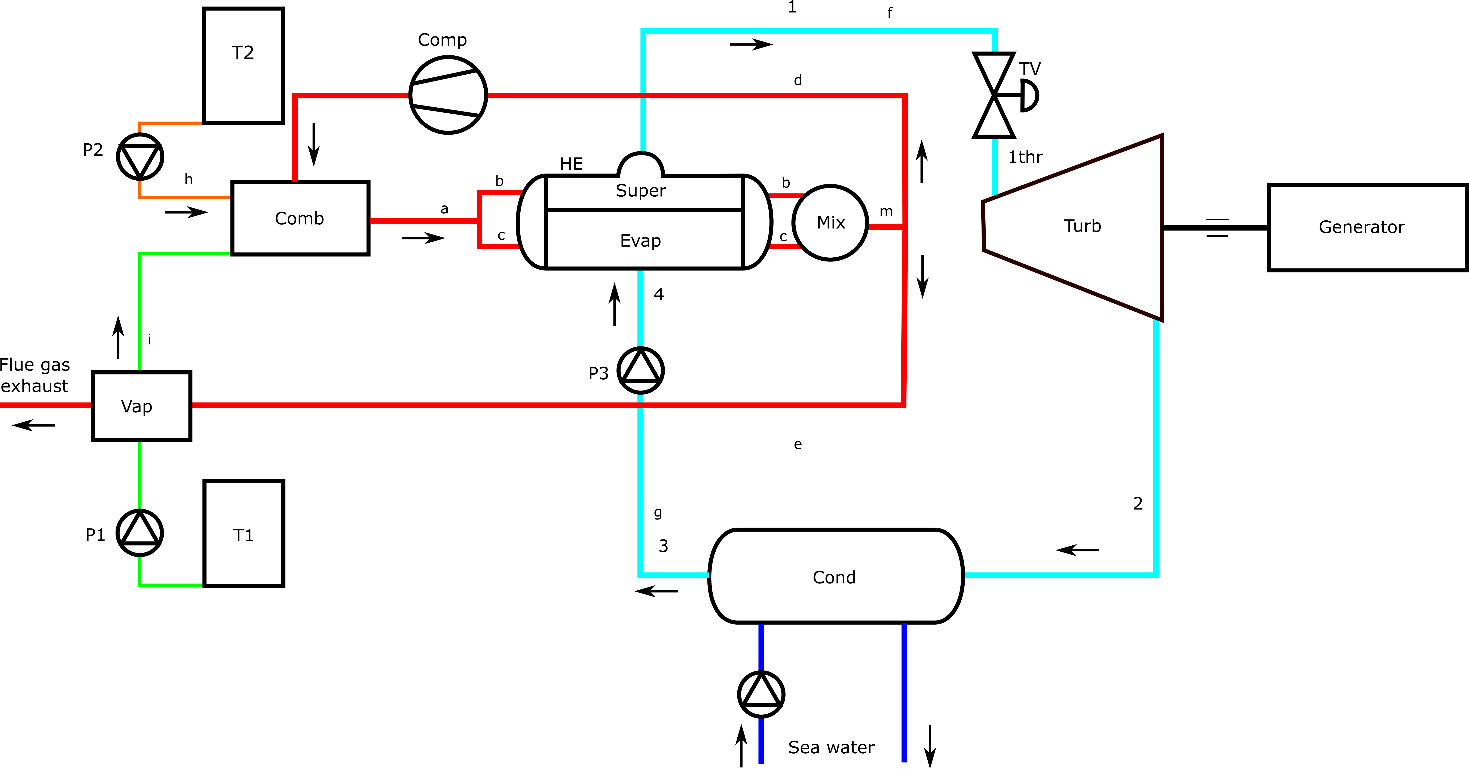
\includegraphics[width=\textwidth]{Thermodynamics/pwr_system.png}
		\caption{Power generation system.}
		\label{fig:pwr_scheme}
	\end{figure}
	
	Submarine power generation system consists of two main circuits; flue gas circuit (red) and steam circuit (cyan). Steam circuit is used for steam production which expands in turbine "Turb" providing necessary power for the "Generator" used for charging the batteries for submarine propulsion. The flue gas circuit is used to provide necessary heat flow for evaporating and superheating the steam for the turbine. Flue gas is generated in the combustion chamber "Comb" in which energy is released by ethanol combustion in pure oxygen.
	
	Liquefied oxygen and ethanol fuel are stored in separate tanks "T1" and "T2", respectively. While pump P2 delivers fuel stream "h" to combustion chamber "Comb", cryogenic pump P2 delivers liquefied oxygen stream "i" to oxygen vaporizer "Vap" where it vaporizes and enters combustion chamber "Comb" in stoichiometric ratio at which fuel combustion is, by assumption, complete without any excess oxygen. Flue gas temperature at the outlet from the combustion chamber (stream "a") is controlled by return stream of cooled flue gas "d" by compressor "Comp" and should never exceed maximum allowed flue gas temperature %ϑ_(fg,max).
	
	Flue gas stream "a", which exits combustion chamber "Comb" enters heat exchanger "HE" used for water evaporation and steam superheating. Therefore, heat exchanger "HE" comprises two sections; an evaporation section "Evap" and superheating section "Super". Total flue gas mass flow which enters heat exchanger "HE" is divided into two flue gas streams "b" and "c". Stream "c" flows through evaporation ("Evap") section and stream "b" flows through superheating ("Super") section in parallel configuration. On heat exchanger exit, two flue gas parallel streams "b" and "c" are adiabatically mixed in mixing chamber "Mix" forming flue gas stream "m".Part of stream "m" is returned by compressor "Comp" to combustion chamber "Comb" as stream "d" to prevent overheating (maximum allowed flue gas temperature), while the rest (stream "e") is used for oxygen evaporation in heat exchanger "Vap" and evacuated outside submarine.
	  
	Heat exchanger "HE" is a pool boiling type apparatus which means that liquid water in the evaporating section is at rest and is evaporated by the flue gas that passes through a tube bundle in the evaporating section. The exact amount of steam that is evaporated in evaporation section "Evap" (which corresponds to the steam mass flow of stream "g") is then superheated in superheating section "Super" of heat exchanger "HE" producing the superheated steam "f". Superheated steam (stream "f") passes through throttling valve "TV" and enters the steam turbine "Turb" where mechanical power is produced by steam adiabatic expansion to condensation pressure p2. After the expansion, low pressure steam condenses in sea water cooled condenser "Cond" and is returned to high pressure evaporator "Evap" by condensate pump "P3". 
	
	The turbine drives an alternator-rectifier which supplies submarine propulsion system with direct current. (?) Required mechanical power for submarine propulsion and auxiliary systems should in every timestep be provided by turbine (no buffer). (dogovor s mentorskim teamom)
	
	Following sections provide a detailed description of every part of power generation system that should be modeled.
	
	\section{Turbine}
	
	A Steam Turbine is a mechanical device in which thermal energy is extracted from pressurized steam by its adiabatic expansion and is transformed to mechanical work.  Therefore, for a given mass flow rate of steam qm, power $P$ generated by steam turbine is defined:
	
	\begin{equation}\label{eq:power}
		P = q_m(h_1 - h_2),
	\end{equation}
	
	where 
	$q_m$ is steam mass flow rate, 
	$h_1$ is steam specific enthalpy at turbine inlet,
	$h_2$ is steam specific enthalpy at turbine outlet.
	Turbine steam swallowing capacity mass flow rate $q_m$ at given pressures and inlet temperature can be expressed by Stodola’s Ellipse equation:
	
	\begin{equation}\label{eq:stodola}
		q_m = \frac{K}{\sqrt(T)}(p_1^2 - p_2^2)^\frac{1}{2},
	\end{equation}
	
	where:
	$K$ is Stodola’s coefficient, 
	$p_1$ is turbine inlet pressure
	$p_2$ is turbine outlet pressure
	$T$ is turbine inlet absolute temperature.
	
	\section{Steam turbine isentropic efficiency}
	
	Turbine isentropic efficiency $\eta$ is defined as the ratio between enthalpy drop at actual turbine expansion and enthalpy drop at isentropic expansion between inlet and outlet turbine pressure $p_1$ and $p_2$.
	
	\begin{equation}\label{eq:eta}
		\eta = \frac{h_1-h_2}{h_1 - h_{2s}}.
	\end{equation}
	
	Steam turbine isentropic efficiency depends upon mean steam volume flow rate qv according to the following equation:
	
	\begin{equation}\label{eq:eta2}
		\eta = aq_v^2 + bq_v + c,
	\end{equation}
	
	\noindent
	where $q_v$ is geometric mean of volume flow rates at turbine inlet ($q_{v,in}$) and at outlet in case of isentropic expansion ($q_{v,out,s}$). 
	
	\begin{equation}\label{eq:q_v}
		q_v = \sqrt{q_{v,in} \cdot q_{v,out,s}},
	\end{equation}
	
	Turbine efficiency is highest at its nominal design point for which pressures (p1, p2) and inlet temperature T1 are given in table 1, while nominal flow rate is defined by Stodola’s ellipse equation \ref{eq:stodola}. Turbine can operate at other conditions (off design turbine performance with lower, i.e. higher mass flow rates than the nominal) with the cost of reduced efficiency, provided that these conditions are not outside permitted values.
	
	\section{Off design turbine performance}
	
	Lower mass flow rate
	
	Steam throttling is a common way for reduction of power produced by steam turbine. By reducing fuel pump “P2" and oxygen pump “P1" speed accordingly when power demand is lowered, fuel consumption and evaporated steam mass flow rate are decreased. In conjunction with steam flow rate decrease, throttling valve “TV" orifice is constricted to reduce turbine inlet pressure $p_{1,thr}$ to a value which satisfies Stodola’s Ellipse law \ref{eq:stodola} for given decreased mass flow rate $q_m$. In a throttling process, superheated steam which exits heat exchanger “HE" is throttled to lower pressure $p_{1,thr}$, while steam enthalpy is conserved. 
	
	
	\section{The Task}
	
	\subsection{Task 1}
	
	\import{Tasks/}{"Task 1"}
	
	\subsection{Task 2}
	
	\import{Tasks/}{"Task 2"}
	
	
	
\end{document}
